% !TeX root = origami-math-en.tex

\appendix


\chapter{GeoGebra links}\label{a.geo}

\begin{center}
\begin{tabular}{|l|l|}
\hline
Axiom 1& \url{https://www.geogebra.org/m/fq9d5hms}\\\hline
Axiom 2& \url{https://www.geogebra.org/m/fgmfss27}\\\hline
Axiom 3& \url{https://www.geogebra.org/m/ek3mqupw}\\\hline
Axiom 4& \url{https://www.geogebra.org/m/renzzbdg}\\\hline
Axiom 5& \url{https://www.geogebra.org/m/aszn9ywu}\\\hline
Axiom 6& \url{https://www.geogebra.org/m/bxe5e5ku}\\\hline
Axiom 7& \url{https://www.geogebra.org/m/yeq5gmeg}\\\hline
Abe's trisection & \url{https://www.geogebra.org/m/dxrcvjam}\\\hline
Martin's trisection & \url{https://www.geogebra.org/m/caky7edd}\\\hline
Messer's doubling of the cube & \url{https://www.geogebra.org/m/mrcwjqh8}\\\hline
Beloch's doubling of the cube & \url{https://www.geogebra.org/m/enzmmwua}\\\hline
\end{tabular}
\end{center}
Due to a bug in Geogebra, in projects that use Axiom~6, points defined by reflection around the common tangent are not saved or are saved incorrectly.

\chapter{Derivation of trigonometric identities}\label{a.tangent}

The trigonometric identifies for tangent used in the proof of Axiom 3 can be derived from identities for the sine and cosine:

\begin{form}{2.2}
\tan (\theta_1+\theta_2) &=& \disfrac{\sin(\theta_1+\theta_2)}{\cos(\theta_1+\theta_2)}\\
&=&\disfrac{\sin\theta_1\cos\theta_2+\cos\theta_1\sin\theta_2}{\cos\theta_1\cos\theta_2-\sin\theta_1\sin\theta_2}\\
&=&\disfrac{\sin\theta_1+\cos\theta_1\tan\theta_2}{\cos\theta_1-\sin\theta_1\tan\theta_2}\\
&=&\disfrac{\tan\theta_1+\tan\theta_2}{1-\tan\theta_1\tan\theta_2}\,.
\end{form}

We use this formula with $\theta=(\theta/2)+(\theta/2)$ to obtain a quadratic equation in $\tan(\theta/2)$:
\begin{form}{2.2}
\tan \theta=\disfrac{\tan(\theta/2)+\tan(\theta/2)}{1-\tan^2(\theta/2)}\\
\tan\theta \,(\tan(\theta/2))^2 \;+\; 2\,(\tan (\theta/2)) \;-\;\tan \theta = 0\,.
\end{form}
Its solutions are:
\[
\tan(\theta/2) = \disfrac{-1\pm\sqrt{1+\tan^2\theta}}{\tan\theta}\,.
\]

\chapter{Parabolas}\label{a.parabola}


Students are usually introduced to parabolas as the graphs of second degree equations $y=ax^2+bx+c$. However, parabolas can be defined geometrically: given a point, the \emph{focus}, and a line, the \emph{directrix}, the locus of points equidistant from the focus and the directrix defines a parabola.


The following diagram shows the focus---the large dot at $p=(0,f)$, and the directrix---the thick line $d$ whose equation is $y=-f$. The resulting parabola is shown as a dotted curve. Its \emph{vertex} $p_2$ is at the origin of the axes.

\begin{center}
\begin{tikzpicture}[scale=1]
\draw (-6,0) -- node[very near start,below,xshift=-32pt] {$x$-\textsf{axis}} (6,0);
\draw (0,-3) -- node[very near start,right,yshift=-20pt] {$y$-\textsf{axis}} (0,4.5);
\draw[ultra thick] (-6,-2) -- node[near start,below] {\textsf{directrix} $d: \quad y=-f$} (6,-2);
\draw[domain=-6:6,samples=50,very thick,dotted] plot (\x,{\x*\x/8});
\coordinate (F) at (0,2);
\fill (F) circle (3pt) node[above left,xshift=-2pt,yshift=15pt] {$(0,f)$} node[above left,xshift=-2pt,yshift=30pt] {\textsf{focus}} node[above right] {$p$};
\fill (0,0) circle (1.5pt) node[below right] {$p_2$};
\fill (0,-2) circle (1.5pt);
\fill (2,-2) circle (1.5pt);
\fill (3,-2) circle (1.5pt);
\fill (5,-2) circle (1.5pt);
\coordinate (FP) at (-5,-2);
\fill (FP) circle (1.5pt) node[below] {$p'$};
\coordinate (F1) at (2,.5);
\fill (F1) circle (1.5pt) node[below right] {$p_3$};
\coordinate (F2) at (3,1.125);
\fill (F2) circle (1.5pt) node[below right] {$p_4$};
\coordinate (F3) at (5,3.125);
\fill (F3) circle (1.5pt) node[below right] {$p_5$};
\coordinate (F4) at (-5,3.125);
\fill (F4) circle (1.5pt) node[above right] {$p_1$};
\draw (F) -- node[left] {$a_2$} (0,0) -- node[left] {$a_2$} (0,-2);
\draw (F) -- node[near end,left] {$a_3$} (F1) -- node[left] {$a_3$} (2,-2);
\draw (F) -- node[near end,above] {$a_4$} (F2) -- node[left] {$a_4$} (3,-2);
\draw (F) -- node[above] {$a_5$} (F3) -- node[left] {$a_5$} (5,-2);
\draw (F) -- node[above] {$a_1$} (F4) -- node[left] {$a_1$} (FP);
\draw[thick,dashed] ($(F4)!-.4!(-2.5,0)$) -- node[very near end,right,xshift=2pt] {$l_1$} ($(F4)!1.8!(-2.5,0)$);
\draw (0,-2) rectangle +(8pt,8pt);
\draw (2,-2) rectangle +(8pt,8pt);
\draw (3,-2) rectangle +(8pt,8pt);
\draw (5,-2) rectangle +(8pt,8pt);
\draw (-5,-2) rectangle +(8pt,8pt);
\end{tikzpicture}
\end{center}

We have selected five points $p_i$, $i=1,\ldots,5$ on the parabola. Each point $p_i$ is at a distance of $a_i$ both from the focus and from the directrix. Drop a perpendicular from $p_i$ to the directrix and let $p_i'$ be the intersection of the perpendicular and the directrix. Using Axiom~2, construct the line $l_i$ by folding $p$ onto $p_i'$. Since $p_i$ is on the parabola, $\overline{p'p_i}=\overline{p_{i}p}=a_i$. The diagram shows the fold $l_1$ through $p_1$. 

\newpage

\textbf{Theorem} The folds are tangents to the parabola.

\textbf{Proof (Oriah Ben Lulu)} 
In the following diagram, the focus is $p$, the directrix is $l$, $p'$ is a point on the directrix and $m$ is the fold that places $p$ on $p'$. By definition, $m$ is the perpendicular bisector of $\overline{pp'}$. Let $s$ be the intersection of $\overline{pp'}$ and $m$; then $\overline{ps}=\overline{p's}=a$ and $m\perp \overline{pp'}$.

\begin{center}
\begin{tikzpicture}[scale=1.1]
\draw[ultra thick] (-6,-2) -- node[near end, below] {$l$} (6,-2);
\draw[domain=-5.5:5.5,samples=50,very thick,dotted] plot (\x,{\x*\x/8});
\coordinate (F) at (0,2);
\fill (F) circle (2pt) node[above right] {$p$};
\coordinate (FP) at (-3,-2);
\fill (FP) circle (1.5pt) node[below] {$p'$};
\coordinate (F4) at (-3,1.125);
\fill (F4) circle (1.5pt) node[above right] {$r$};
\coordinate (F5) at (-5,2.775);
\fill (F5) circle (1.5pt) node[left,yshift=-4pt] {$q$};
\coordinate (F5p) at (-5,-2);
\fill (F5p) circle (1.5pt) node[below] {$p''$};
\draw (F) -- node[above] {$b$} (F4) -- node[left] {$b$} (FP);
\draw (F) -- node[above] {$c$} (F5);
\draw (F5) -- node[left] {$d$} (F5p);
\draw[thick,dashed,name path=fold] ($(F4)+(140:4)$) -- (F4) -- node[below,xshift=-2pt,yshift=-2pt] {$m$} ($(F4)+(-40:5.1)$);
\draw (FP) rectangle +(8pt,8pt);
\draw (F5p) rectangle +(8pt,8pt);
\draw (F5) -- (FP);
\draw[name path=base] (F) -- (FP);
\path [name intersections = {of = base and fold, by = {G}}];
\fill (G) circle (1.5pt) node[below,yshift=-4pt] {$s$};
\draw[rotate=140] (G) rectangle +(6pt,6pt);
\path (FP) -- node[left] {$c$} (F5);
\path (F) -- node[below] {$a$} (G) -- node[below] {$a$} (FP);
\end{tikzpicture}
\end{center}
Let $r$ be the intersection of a perpendicular to $l$ through $p'$ and the fold $m$. Then $\triangle psr\cong \triangle p'sr$ by side-angle-side, since $\overline{ps}=\overline{p's}$,  $\angle psr=\angle p'sr=90^\circ$ and $\overline{rs}$ is a common edge. It follows that $\overline{pr}=\overline{p'r}=b$ and therefore $r$ must be on the parabola.

Choose a point $p''$ on the directrix that is \emph{distinct} from $p'$ and suppose that $m$ is also the fold that places $p$ on $p''$. Let $q$ be the intersection of the perpendicular to $l$ through $p''$ and the fold $m$. As before, we can prove that $\overline{pq}=\overline{p'q}=c$. Let $\overline{qp''}=d$. If $q$ is on the parabola then $d=\overline{qp''}=\overline{qp}=c$. But $c$ is the hypotenuse of the right triangle $\triangle qp''p'$ and cannot be equal to one of its sides $d$.

We have proved that $m$ intersects the parabola in only one point so it is a tangent to the parabola.

\chapter{Tangents Common to Two Parabolas}\label{a.number-of-tangents}

Here are diagrams showing the four cases:

\bigskip\bigskip

\begin{center}
\begin{tikzpicture}[scale=.8]
\draw (-7,0) -- (7,0);
\draw (0,-1) -- (0,7);
\coordinate (P1) at (0,6);
\fill (P1) circle (2pt) node[above left] {$p_1$};
\coordinate (P2) at (0,2);
\fill (P2) circle (2pt) node[above left] {$p_2$};
\draw[thick] (-7,3) -- node[very near start,above,xshift=-25pt] {$l_1$} (7,3);
\draw[thick] (-7,1) -- node[very near start,above,xshift=-25pt] {$l_2$} (7,1);
\draw[domain=-3.1:3.1,samples=50,very thick,dotted] plot (\x,{.25*\x*\x+4.5});
\draw[domain=-4.5:4.5,samples=50,very thick,dotted] plot (\x,{.25*\x*\x+1.5});
\end{tikzpicture}
\end{center}

\bigskip\bigskip

\begin{center}
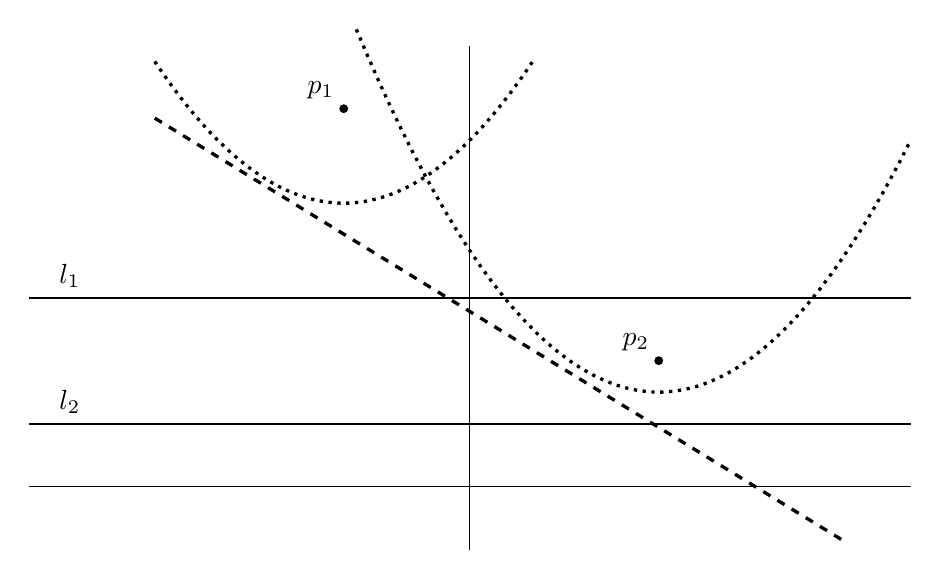
\begin{tikzpicture}[scale=.8]
\draw (-7,0) -- (7,0);
\draw (0,-1) -- (0,7);
\coordinate (P1) at (-2,6);
\fill (P1) circle (2pt) node[above left] {$p_1$};
\coordinate (P2) at (3,2);
\fill (P2) circle (2pt) node[above left] {$p_2$};
\draw[thick] (-7,3) -- node[very near start,above,xshift=-25pt] {$l_1$} (7,3);
\draw[thick] (-7,1) -- node[very near start,above,xshift=-25pt] {$l_2$} (7,1);
\draw[domain=-5:1,samples=50,very thick,dotted] plot (\x,{.25*(\x+2)*(\x+2)+4.5});
\draw[domain=-1.8:7,samples=50,very thick,dotted] plot (\x,{.25*(\x-3)*(\x-3)+1.5});
\draw[very thick,dashed] (-5,5.85) -- (6,-.9);
\end{tikzpicture}
\end{center}

\bigskip\bigskip

\begin{center}
\begin{tikzpicture}[scale=.8]
\draw (-7,0) -- (7,0);
\draw (0,-7) -- (0,5);
\coordinate (P1) at (0,4);
\fill (P1) circle (2pt) node[above left] {$p_1$};
\coordinate (P2) at (0,-6);
\fill (P2) circle (2pt) node[above left] {$p_2$};
\draw[thick] (-7,2) -- node[very near start,above,xshift=-25pt] {$l_1$} (7,2);
\draw[thick] (-7,-2) -- node[very near start,below,xshift=-25pt] {$l_2$} (7,-2);
\draw[domain=-4.8:4.8,samples=50,very thick,dotted] plot (\x,{-.13*\x*\x-4});
\draw[domain=-2.8:2.8,samples=50,very thick,dotted] plot (\x,{.25*\x*\x+3});
\draw[very thick,dashed] (-5,-7) -- (2.95,5);
\draw[very thick,dashed] (-3,5) -- (4.95,-7);
\end{tikzpicture}
\end{center}

\bigskip\bigskip

\begin{center}
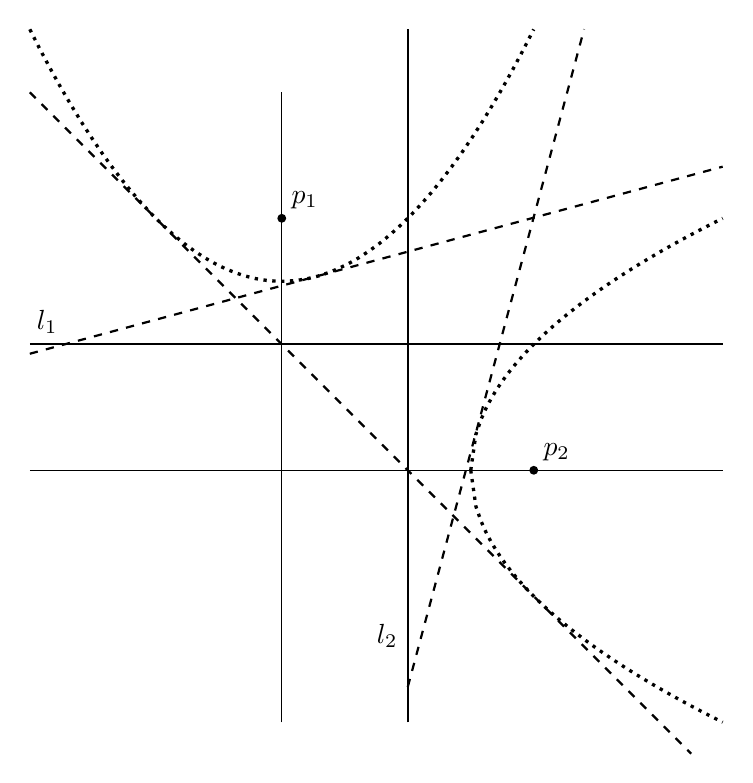
\begin{tikzpicture}[scale=.8]
\draw (-4,0) -- (7,0);
\draw (0,-4) -- (0,6);
\coordinate (P1) at (0,4);
\fill (P1) circle (2pt) node[above right] {$p_1$};
\coordinate (P2) at (4,0);
\fill (P2) circle (2pt) node[above right] {$p_2$};
\draw[thick] (-4,2) -- node[very near start,above,xshift=-25pt] {$l_1$} (7,2);
\draw[thick] (2,-4) -- node[very near start,left] {$l_2$} (2,7);
\draw[domain=-4:4,samples=50,very thick,dotted] plot (\x,{.25*\x*\x+3});
\draw[domain=3:7,samples=50,very thick,dotted] plot (\x,{sqrt(4*\x-12)});
\draw[domain=3:7,samples=50,very thick,dotted] plot (\x,{-sqrt(4*\x-12)});

\draw[thick,dashed,domain=-4:6.5] plot (\x,-\x+2);
\draw[thick,dashed,domain=-4:7] plot (\x,.27*\x+2.93);
\draw[thick,dashed,domain=2:4.8] plot (\x,3.73*\x-10.9);
\end{tikzpicture}
\end{center}

